% ============================================================
% Revised draft after the 3 Nov 2026 supervisor review.
% This file addresses the text-only comments (priority A).
% It does NOT contain new experiments (priority B/C). Those are
% listed as future work and in the notes at the end of this file.
%
% Still to fill before submission (search for TODO):
%   * co-author names and emails (or delete the extra author blocks)
%   * four real dataset images in paper/figs/
% Page limit: 6 pages including references. Check after the images
% are inserted.
%
% Rounding rule used everywhere:
%   means are the logged means, shown to 3 decimals;
%   every drop is (unrounded mean_dense - unrounded mean_pruned),
%   then rounded to 3 decimals;
%   ± is the SAMPLE std (divisor n-1). The logs store the population
%   std (divisor n). We multiply by sqrt(n/(n-1)). For n=3 that
%   factor is sqrt(3/2). Two-seed rows have no ±.
% No AI-generated images. The curves and the pipeline are TikZ.
% ============================================================
\documentclass[conference]{IEEEtran}
\IEEEoverridecommandlockouts

\usepackage{cite}
\usepackage{amsmath,amssymb,amsfonts}
\usepackage{graphicx}
\usepackage{booktabs}
\usepackage{xcolor}
\usepackage{textcomp}
\usepackage{url}
\usepackage{pgfplots}
\pgfplotsset{compat=1.16}
\usepgfplotslibrary{groupplots}
\usetikzlibrary{calc,arrows.meta,positioning}

\newcommand{\TODO}[1]{\textcolor{red}{[TODO: #1]}}

% Real photos go in paper/figs/. Until then a labeled box is shown.
\newcommand{\sampleorbox}[2]{%
  \begin{minipage}[c][2.15cm][c]{0.23\textwidth}
    \centering
    \IfFileExists{#1}{%
      \includegraphics[width=\linewidth,height=2.0cm,keepaspectratio]{#1}}{%
      \fbox{\parbox[c][1.85cm][c]{0.90\linewidth}{\centering\scriptsize #2}}}
  \end{minipage}}

\begin{document}

\title{Does Compressibility Transfer Across Datasets?\\
A Study of CNN Pruning for Optical UAV and SAR Flood Classification}

\author{\IEEEauthorblockN{Abdul Rauf}
\IEEEauthorblockA{\textit{Faculty of Computer Science and Engineering} \\
\textit{GIK Institute of Engineering Sciences and Technology}\\
Topi, Pakistan \\
u2024020@giki.edu.pk}
\and
\IEEEauthorblockN{\TODO{2nd author}}
\IEEEauthorblockA{\textit{Faculty of Computer Science and Engineering} \\
\textit{GIK Institute of Engineering Sciences and Technology}\\
Topi, Pakistan \\
\TODO{email}}
\and
\IEEEauthorblockN{\TODO{3rd author}}
\IEEEauthorblockA{\textit{Faculty of Computer Science and Engineering} \\
\textit{GIK Institute of Engineering Sciences and Technology}\\
Topi, Pakistan \\
\TODO{email}}
\and
\IEEEauthorblockN{\TODO{4th author}}
\IEEEauthorblockA{\textit{Faculty of Computer Science and Engineering} \\
\textit{GIK Institute of Engineering Sciences and Technology}\\
Topi, Pakistan \\
\TODO{email}}
}

\maketitle

\begin{abstract}
Magnitude pruning is a common way to run convolutional networks on the
small platforms used in disaster response, but it is usually tested
only on optical images. We ask whether the same compression still holds
on a second flood dataset. One supervised pipeline trains ResNet18 and
VGG-16 on FloodNet (optical UAV imagery) and Sen1Floods11 (Sentinel-1
SAR). SAR chips are labeled by a water-fraction rule, and every number
uses a split of the labeled images. We apply global unstructured and
filter-wise structured $L_1$ pruning, then fine-tune every setting the
same way. Over three seeds (96 runs) we report final-epoch accuracy,
balanced accuracy, macro-F1, and AUC. On these two datasets,
unstructured pruning transfers: at 90\% sparsity ResNet18 loses at most
$0.03$ macro-F1 on both. Structured pruning does not. At 50\%, FloodNet
loses less than $0.001$ macro-F1 and Sen1Floods11 loses $0.067$, and
the gap grows with the ratio. A lower fine-tuning learning rate does
not close it. VGG-16 is unstable: one dense SAR seed fails while AUC
stays near $0.858$, and several structured runs collapse. A sparsity
budget checked on one of these datasets should be checked again on the
other.
\end{abstract}

\begin{IEEEkeywords}
network pruning, model compression, flood detection, SAR, optical
remote sensing, FloodNet, Sen1Floods11
\end{IEEEkeywords}

\section{Introduction}
Flood maps are needed within hours, often on a small UAV, an edge box,
or a nanosatellite that cannot host a large network
\cite{rahnemoonfar2021floodnet,khan2023floodresnet50}. Magnitude
pruning removes small weights or whole filters and then fine-tunes the
network \cite{han2015learning,li2017pruning,hoefler2021sparsity}. On
optical benchmarks this often keeps accuracy at high sparsity
\cite{blalock2020state}. Those tests are usually run on one dataset.
A model compressed for optical UAV images may later be asked to read
Sentinel-1 SAR, which is the sensor that still sees the ground through
cloud \cite{bonafilia2020sen1floods11}.

This paper asks one question:
\begin{quote}
\emph{Does a heavily pruned classic CNN hold its accuracy on both an
optical UAV flood dataset and a SAR flood dataset, or does one dataset
break down while the other does not?}
\end{quote}
We do not claim a general law about sensors. FloodNet and Sen1Floods11
also differ in size, resolution, class balance, and how the labels were
made. The controlled part of the study is the pipeline: the same
architectures, input size, augmentation, sampler, optimizer, schedule,
pruning operators, ratios, and fine-tuning budget, with only the
dataset changed.

The backbones are ResNet18 (11.18M parameters) \cite{he2016resnet} and
VGG-16 (134.3M) \cite{simonyan2015vgg}. Sen1Floods11 is labeled per
pixel. We turn each hand-labeled mask into one image label with the
rule in Section~\ref{sec:setup}. That positive class means ``at least
1\% of the valid pixels are water.'' The mask includes permanent water
(rivers and lakes). We did not remove it, so the SAR label is not a
confirmed flood label.

\noindent\textbf{Contributions.}
\begin{itemize}
\item A 96-run study (two architectures, two datasets, two pruning
families, several ratios, three seeds) with the training pipeline held
fixed.
\item An explicit rule that turns Sen1Floods11 water masks into
image-level labels so they can be scored like FloodNet. The code
and split lists are released (see the conclusion).
\item On these two datasets, unstructured pruning of ResNet18 costs at
most $0.03$ macro-F1 at 90\% sparsity, while 50\% structured pruning
costs less than $0.001$ on FloodNet and $0.067$ on Sen1Floods11.
A lower fine-tuning learning rate, within the range we tested, does
not remove that gap.
\item VGG-16 as an instability case: one dense SAR seed fails at the
final-epoch threshold while AUC stays near $0.858$, and structured
runs collapse on both datasets. This is consistent with a serial
network that has no skip connections and no BatchNorm; we do not claim
that missing skips are the only cause.
\end{itemize}

\section{Related Work}
\subsection{Datasets and Flood Classifiers}
FloodNet \cite{rahnemoonfar2021floodnet} is UAV imagery from Hurricane
Harvey. Its Track-1 classification split has 398 labeled training
images (51 flooded, 347 non-flooded). The official validation and test
classification labels were withheld, so any labeled score has to come
from those 398 images. Sen1Floods11 \cite{bonafilia2020sen1floods11}
has $512\times512$ Sentinel-1 chips from 11 flood events, with 446
hand-labeled chips. The mask values are water, non-water, and invalid.
It is a segmentation dataset. CNN flood mapping on Sentinel-1 is
usually done at pixel level \cite{nemni2020flood}; we instead score a
single label per chip so the pruning comparison matches FloodNet.

Khose \emph{et al.} \cite{khose2021semisupervised} report 96.70\% test
accuracy for a semi-supervised ResNet18 (11.6M parameters) on FloodNet,
using pseudo-labels \cite{lee2013pseudo}. We use supervised training
only, so pruning is not mixed with pseudo-label noise. Khan \emph{et
al.} \cite{khan2023floodresnet50} report 96.43\% accuracy and 86.36\%
F1 for Flood-ResNet50 (98\,MB, 4.3 billion FLOPs) on a Jetson Nano.
Their F1 is not our macro-F1. Both published scores use the hidden
FloodNet test set. Our dense ResNet18 reaches 97.0\% accuracy and
0.929 macro-F1 on a 199-image split of the labeled training images.
Those numbers are not directly comparable.

\subsection{Pruning}
Unstructured magnitude pruning zeros individual weights
\cite{han2015learning}. It needs sparse kernels to become faster.
Structured pruning removes whole filters \cite{li2017pruning}, which
runs on ordinary hardware, but it is a coarser choice. Channel pruning
\cite{he2017channel} and Taylor-based filter pruning
\cite{molchanov2017pruning} are other structured criteria; we use the
$L_1$ norm because it is simple and identical on both datasets.
Later work argues that pruning mostly reveals a trainable subnetwork
\cite{frankle2019lottery} or a better architecture
\cite{liu2019rethinking}, and that papers test these ideas on a few
optical benchmarks with incompatible protocols
\cite{blalock2020state,hoefler2021sparsity}. Compression can also hurt
some examples much more than the average accuracy shows
\cite{hooker2019forget}. That matters here: flooded images are 12.8\%
of FloodNet and 66.4\% of our Sen1Floods11 labels, so accuracy alone
can hide a class that collapsed.

Pruning has been used inside remote sensing, but on one dataset at a
time: channel pruning for optical scene classification
\cite{wei2022nasprune}, and filter pruning plus distillation for SAR
target recognition \cite{wang2021sarprune}. We did not find a study
that freezes the flood-classification pipeline and changes only the
dataset. That is the comparison we run.

\section{Experimental Setup}
\label{sec:setup}

\begin{figure*}[t]
\centering
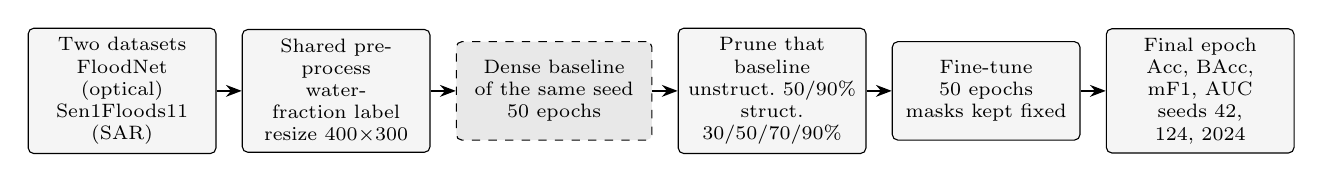
\begin{tikzpicture}[
  font=\scriptsize,
  box/.style={draw, rounded corners=2pt, align=center,
              minimum height=1.25cm, text width=2.15cm, fill=gray!8},
  dbox/.style={draw, dashed, rounded corners=2pt, align=center,
              minimum height=1.25cm, text width=2.25cm, fill=gray!18},
  arr/.style={-{Stealth[length=2mm]}, thick}]
\node[box] (data) {Two datasets\\FloodNet (optical)\\Sen1Floods11 (SAR)};
\node[box, right=0.32cm of data] (prep) {Shared preprocess\\water-fraction label\\resize $400{\times}300$};
\node[dbox, right=0.32cm of prep] (dense) {Dense baseline\\of the same seed\\50 epochs};
\node[box, right=0.32cm of dense] (prune) {Prune that baseline\\unstruct.\ 50/90\%\\struct.\ 30/50/70/90\%};
\node[box, right=0.32cm of prune] (ft) {Fine-tune\\50 epochs\\masks kept fixed};
\node[box, right=0.32cm of ft] (eval) {Final epoch\\Acc, BAcc, mF1, AUC\\seeds 42, 124, 2024};
\draw[arr] (data) -- (prep);
\draw[arr] (prep) -- (dense);
\draw[arr] (dense) -- (prune);
\draw[arr] (prune) -- (ft);
\draw[arr] (ft) -- (eval);
\end{tikzpicture}
\caption{Study pipeline. The dashed box is the dense checkpoint of the
same seed; every pruned run starts from it. Architecture, resolution,
augmentation, sampler, optimizer, schedule, operators, ratios, and
fine-tuning budget stay fixed. Only the dataset changes.}
\label{fig:pipeline}
\end{figure*}

Fig.~\ref{fig:pipeline} is the whole study. Table~\ref{tab:datasets}
lists the data actually used.

\begin{table}[t]
\centering
\caption{Data used in this study. Sizes are width$\times$height.}
\label{tab:datasets}
\footnotesize
\setlength{\tabcolsep}{3.2pt}
\begin{tabular}{lcc}
\toprule
 & \textbf{FloodNet} & \textbf{Sen1Floods11}\\
\midrule
Sensor & UAV, RGB & Sentinel-1, VV+VH\\
Original size & $4000{\times}3000$ & $512{\times}512$\\
Network input & $400{\times}300$ & $400{\times}300$\\
Labeled images & 398 & 441\\
Train / validation & 199 / 199 & 220 / 221\\
Positive class & 12.8\% flooded & 66.4\% water\\
How labeled & image label & mask, $\tau{=}1\%$\\
\bottomrule
\end{tabular}
\end{table}

\subsection{Labels and Inputs}
FloodNet images are $4000\times3000$ (width$\times$height). We resize
them to $400\times300$, which keeps the $4{:}3$ frame. The 398 labeled
images are split 50/50, stratified, with data seed 42 (199/199). This
follows the public baseline's use of the labeled training images
\cite{khose2021semisupervised}, because the official test labels are
hidden. The validation half contains about 25 flooded images.

For each Sen1Floods11 chip we compute
\begin{equation}
y = \mathbf{1}\!\left[\frac{\left|\{p : m_p = 1\}\right|}
{\left|\{p : m_p \neq -1\}\right|} \;\geq\; \tau\right],
\qquad \tau = 0.01,
\label{eq:labelconv}
\end{equation}
and drop chips with no valid pixels. A positive chip has at least 1\%
water among valid pixels. At this threshold a river is enough to count
as positive, and permanent water was not removed, so $y{=}1$ means
``contains water,'' not ``flooded.'' The same rule yields 441 chips
(293 positive / 148 negative), split 50/50 stratified with the same
data seed (220/221). The split is by chip, not by flood event, so
neighboring chips from one event can fall on both sides. We treat that
as a limitation, not as a solved robustness check.

SAR backscatter is clipped to $[-50,1]$\,dB, scaled to $[0,1]$, and
stacked as $(\mathrm{VV},\mathrm{VH},(\mathrm{VV}{+}\mathrm{VH})/2)$.
The same clip, scale, and ImageNet normalization are used for training
and validation. Chips are $512\times512$ and are resized to
$400\times300$ so both datasets share one input tensor. That changes
the SAR aspect ratio from $1{:}1$ to $4{:}3$.

\begin{figure*}[t]
\centering
\sampleorbox{figs/floodnet_flooded.jpg}{Add real file:\\figs/floodnet\_flooded.jpg\\FloodNet, flooded}
\hfill
\sampleorbox{figs/floodnet_dry.jpg}{Add real file:\\figs/floodnet\_dry.jpg\\FloodNet, non-flooded}
\hfill
\sampleorbox{figs/s1_chip.png}{Add real file:\\figs/s1\_chip.png\\SAR chip, VV / VH / mean}
\hfill
\sampleorbox{figs/s1_mask.png}{Add real file:\\figs/s1\_mask.png\\same chip, water mask}
\caption{Real examples, not synthetic images. Left pair: FloodNet.
Right pair: one Sen1Floods11 chip as a three-channel composite and its
water mask. Prefer a chip whose water fraction is near 1--3\%, so the
$\tau{=}0.01$ rule is visible. Export each file under 300\,KB and place
it in \texttt{paper/figs/}.}
\label{fig:samples}
\end{figure*}

The class imbalance runs in opposite directions
(Table~\ref{tab:datasets}). We therefore report balanced accuracy and
macro-F1 with accuracy and AUC, and we compare each pruned model only
with its own dense baseline.

\subsection{Training}
Every dense run and every fine-tune uses ImageNet initialization
\cite{deng2009imagenet}, a 2-logit head, unweighted cross-entropy, and
a class-balanced weighted sampler. The only augmentation is random
horizontal and vertical flips. The optimizer is SGD with learning rate
$0.01$, momentum $0$, and weight decay $0$. This recipe is unusual. We
keep it because the study holds one recipe fixed; we do not claim it is
the best optimizer for SAR. Each run lasts 50 epochs. We score the last
epoch, with no early stopping and no best-validation checkpoint.
Seeds 42, 124, and 2024 change initialization, sampling, and
augmentation. The split does not change. Batch size is 64 for ResNet18
and 16 for VGG-16, and it is the same on both datasets.
ResNet18 BatchNorm layers stay in train mode during fine-tuning and in
eval mode at test time. Torchvision VGG-16 has no BatchNorm.
All 96 runs were executed on Kaggle with the free \emph{GPU T4 x2}
accelerator: two NVIDIA Tesla T4 GPUs are attached to that session, and
each model was trained on one of them.
Throughout, $\pm$ is the sample standard deviation over the three seeds.
The logs store the population standard deviation; we rescale by
$\sqrt{3/2}$.

\subsection{Pruning}
Each pruned run loads the dense checkpoint of the same seed.
\begin{itemize}
\item \textbf{Global unstructured $L_1$} \cite{han2015learning}.
Weights of every convolution and linear layer are ranked together, and
the smallest fraction $r\in\{0.5,0.9\}$ is zeroed. Biases are not
pruned.
\item \textbf{Layer-wise structured $L_1$} \cite{li2017pruning}.
In every convolution with more than 8 output channels, and every linear
layer with more than 8 outputs, the fraction
$r\in\{0.3,0.5,0.7,0.9\}$ of filters (or rows) with the smallest $L_1$
norm is masked. The 2-logit classifier is never pruned.
\end{itemize}
The two families are not the same intervention. Structured pruning uses
one ratio in every eligible layer. Unstructured pruning spends the
budget wherever the global magnitude is smallest. They differ in
granularity and in how sparsity is spread across layers.

Masks stay fixed for 50 fine-tuning epochs at learning rate $0.01$.
A control repeats ResNet18 at 50\% and 90\%, and VGG-16 at 70\%, on both
datasets, at learning rate $0.001$ for two seeds (42 and 124) and the
same 50 epochs. That control is a lower rate only. It is a short
schedule with no momentum, so it cannot show that the gap survives a
stronger recipe. We report its mean and no standard deviation, because
two seeds do not support one. The full grid is 12 dense, 48 structured,
24 unstructured, and 12 learning-rate runs.

Two implementation facts change how the parameter counts should be
read. First, structured pruning masks output filters only. The next
layer still has its input channels, and BatchNorm scale and bias on a
masked ResNet filter are not removed. A zeroed convolution followed by
BatchNorm can still emit a constant, so the channel is not physically
gone. The horizontal axis of Fig.~\ref{fig:curves} is the count of
remaining stored parameters, including unpruned biases and BatchNorm
terms. It is not a FLOP count and not the size after deleting channels.
At 50\% both families report 5.59M remaining parameters for that
reason; a network with the channels actually deleted would be smaller.
Second, ResNet18's parameter-free identity shortcuts are not pruned.
Its $1\times1$ projection shortcuts are convolutions with 128, 256, or
512 outputs, so the same structured rule does prune them.

\section{Results and Discussion}
\label{sec:results}

\begin{table}[t]
\centering
\caption{ResNet18, final epoch, mean $\pm$ sample std over 3 seeds.
Par.\ is remaining stored parameters in millions, not physical
channel-removed size. FT learning rate $0.01$.}
\label{tab:resnet}
\footnotesize
\setlength{\tabcolsep}{3.2pt}
\begin{tabular}{llr cc cc}
\toprule
& & & \multicolumn{2}{c}{\textbf{FloodNet}} &
\multicolumn{2}{c}{\textbf{Sen1Floods11}}\\
\cmidrule(lr){4-5}\cmidrule(lr){6-7}
\textbf{Method} & \textbf{Ratio} & \textbf{Par.} &
\textbf{mF1} & \textbf{AUC} & \textbf{mF1} & \textbf{AUC}\\
\midrule
dense      & 0\%  & 11.18 & .929$\pm$.013 & .991$\pm$.003 & .827$\pm$.011 & .908$\pm$.016\\
unstruct.  & 50\% &  5.59 & .917$\pm$.012 & .995$\pm$.002 & .833$\pm$.008 & .912$\pm$.014\\
unstruct.  & 90\% &  1.13 & .911$\pm$.011 & .989$\pm$.002 & .799$\pm$.016 & .888$\pm$.021\\
structured & 30\% &  7.82 & .925$\pm$.014 & .986$\pm$.015 & .768$\pm$.037 & .858$\pm$.019\\
structured & 50\% &  5.59 & .928$\pm$.020 & .989$\pm$.005 & .759$\pm$.008 & .841$\pm$.012\\
structured & 70\% &  3.37 & .857$\pm$.077 & .930$\pm$.063 & .734$\pm$.034 & .834$\pm$.015\\
structured & 90\% &  1.13 & .798$\pm$.078 & .930$\pm$.022 & .577$\pm$.047 & .763$\pm$.032\\
\bottomrule
\end{tabular}
\end{table}

\begin{table}[t]
\centering
\caption{ResNet18 accuracy and balanced accuracy, same runs as
Table~\ref{tab:resnet}. Means over 3 seeds, sample std.}
\label{tab:acc}
\footnotesize
\setlength{\tabcolsep}{3.2pt}
\begin{tabular}{llcccc}
\toprule
& & \multicolumn{2}{c}{\textbf{FloodNet}} &
\multicolumn{2}{c}{\textbf{Sen1Floods11}}\\
\cmidrule(lr){3-4}\cmidrule(lr){5-6}
\textbf{Method} & \textbf{Ratio} & \textbf{Acc} & \textbf{BAcc} &
\textbf{Acc} & \textbf{BAcc}\\
\midrule
dense     & 0\%  & .970$\pm$.005 & .914$\pm$.020 & .840$\pm$.011 & .840$\pm$.009\\
unstruct. & 90\% & .960$\pm$.005 & .920$\pm$.012 & .815$\pm$.016 & .811$\pm$.016\\
struct.   & 50\% & .970$\pm$.009 & .909$\pm$.013 & .780$\pm$.007 & .767$\pm$.010\\
struct.   & 90\% & .893$\pm$.072 & .836$\pm$.058 & .578$\pm$.047 & .656$\pm$.044\\
\bottomrule
\end{tabular}
\end{table}

\begin{table}[t]
\centering
\caption{ResNet18 structured pruning, macro-F1. The $0.01$ column is
3 seeds. The $0.001$ column is the mean of 2 seeds and has no std.
The lower rate does not restore Sen1Floods11.}
\label{tab:lrcontrol}
\footnotesize
\begin{tabular}{llcc}
\toprule
\textbf{Dataset} & \textbf{Ratio} & \textbf{mF1, lr 0.01} &
\textbf{mF1, lr 0.001}\\
\midrule
FloodNet     & 50\% & .928$\pm$.020 & .914\\
FloodNet     & 90\% & .798$\pm$.078 & .699\\
Sen1Floods11 & 50\% & .759$\pm$.008 & .718\\
Sen1Floods11 & 90\% & .577$\pm$.047 & .609\\
\bottomrule
\end{tabular}
\end{table}

\begin{figure*}[t]
\centering
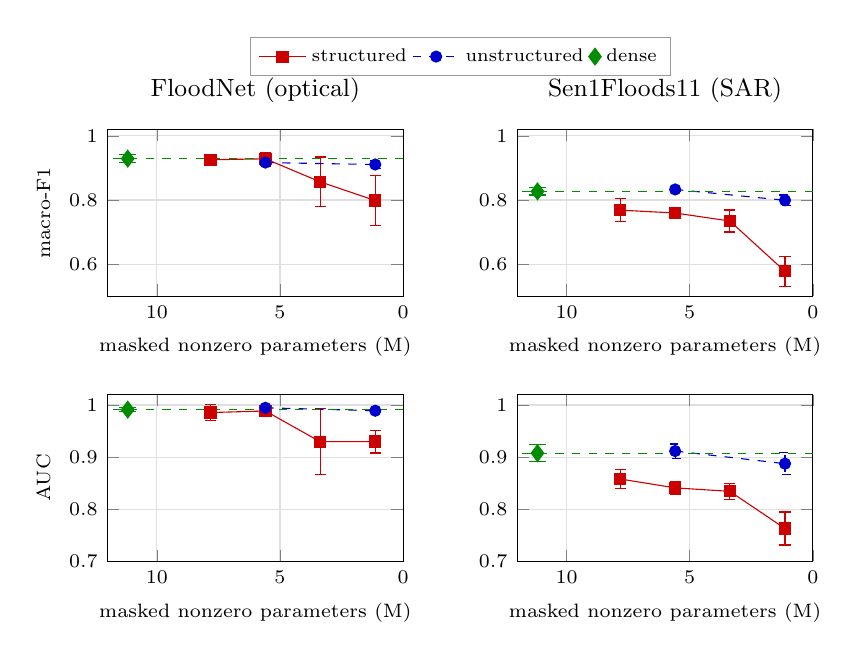
\begin{tikzpicture}
\begin{groupplot}[
  group style={group size=2 by 2, horizontal sep=1.45cm,
               vertical sep=1.25cm},
  width=0.44\textwidth, height=3.7cm,
  x dir=reverse, xmin=0, xmax=12,
  xlabel={masked nonzero parameters (M)},
  grid=major, grid style={gray!25},
  tick label style={font=\scriptsize},
  label style={font=\scriptsize},
  title style={font=\small},
  legend cell align={left},
  legend style={font=\scriptsize, draw=black!40,
                nodes={scale=0.95, transform shape}},
  error bars/y dir=both, error bars/y explicit,
]
\nextgroupplot[title={FloodNet (optical)}, ylabel={macro-F1},
               ymin=0.50, ymax=1.02,
               legend to name=sharedlegend, legend columns=3]
\addplot[mark=square*, solid, color=red!80!black, mark options={solid,fill=red!80!black}]
  coordinates {
 (7.82,0.9253) +- (0,0.0143) (5.59,0.9283) +- (0,0.0196)
 (3.37,0.8566) +- (0,0.0772) (1.13,0.7981) +- (0,0.0781)};
\addlegendentry{structured}
\addplot[mark=*, dashed, color=blue!80!black, mark options={solid,fill=blue!80!black}]
  coordinates {
 (5.59,0.9166) +- (0,0.0119) (1.13,0.9105) +- (0,0.0113)};
\addlegendentry{unstructured}
\addplot[only marks, mark=diamond*, mark size=3pt, color=green!55!black, mark options={solid,fill=green!55!black}]
  coordinates {(11.18,0.9288) +- (0,0.0131)};
\addlegendentry{dense}
\addplot[dashed, color=green!55!black, domain=0:12] {0.9288};
\nextgroupplot[title={Sen1Floods11 (SAR)}, ymin=0.50, ymax=1.02]
\addplot[mark=square*, solid, color=red!80!black, mark options={solid,fill=red!80!black}]
  coordinates {
 (7.82,0.7683) +- (0,0.0365) (5.59,0.7593) +- (0,0.0076)
 (3.37,0.7344) +- (0,0.0343) (1.13,0.5774) +- (0,0.0468)};
\addplot[mark=*, dashed, color=blue!80!black, mark options={solid,fill=blue!80!black}]
  coordinates {
 (5.59,0.8328) +- (0,0.0076) (1.13,0.7990) +- (0,0.0164)};
\addplot[only marks, mark=diamond*, mark size=3pt, color=green!55!black, mark options={solid,fill=green!55!black}]
  coordinates {(11.18,0.8267) +- (0,0.0111)};
\addplot[dashed, color=green!55!black, domain=0:12] {0.8267};
\nextgroupplot[ylabel={AUC}, ymin=0.70, ymax=1.02]
\addplot[mark=square*, solid, color=red!80!black, mark options={solid,fill=red!80!black}]
  coordinates {
 (7.82,0.9856) +- (0,0.0148) (5.59,0.9886) +- (0,0.0051)
 (3.37,0.9297) +- (0,0.0631) (1.13,0.9299) +- (0,0.0220)};
\addplot[mark=*, dashed, color=blue!80!black, mark options={solid,fill=blue!80!black}]
  coordinates {
 (5.59,0.9947) +- (0,0.0020) (1.13,0.9891) +- (0,0.0022)};
\addplot[only marks, mark=diamond*, mark size=3pt, color=green!55!black, mark options={solid,fill=green!55!black}]
  coordinates {(11.18,0.9912) +- (0,0.0034)};
\addplot[dashed, color=green!55!black, domain=0:12] {0.9912};
\nextgroupplot[ymin=0.70, ymax=1.02]
\addplot[mark=square*, solid, color=red!80!black, mark options={solid,fill=red!80!black}]
  coordinates {
 (7.82,0.8581) +- (0,0.0189) (5.59,0.8411) +- (0,0.0118)
 (3.37,0.8344) +- (0,0.0153) (1.13,0.7631) +- (0,0.0316)};
\addplot[mark=*, dashed, color=blue!80!black, mark options={solid,fill=blue!80!black}]
  coordinates {
 (5.59,0.9117) +- (0,0.0135) (1.13,0.8875) +- (0,0.0207)};
\addplot[only marks, mark=diamond*, mark size=3pt, color=green!55!black, mark options={solid,fill=green!55!black}]
  coordinates {(11.18,0.9077) +- (0,0.0160)};
\addplot[dashed, color=green!55!black, domain=0:12] {0.9077};
\end{groupplot}
\node[anchor=south] at ($(group c1r1.north east)!0.5!(group c2r1.north west)+(0,0.55cm)$)
  {\pgfplotslegendfromname{sharedlegend}};
\end{tikzpicture}
\caption{ResNet18 macro-F1 (top) and AUC (bottom) against masked
nonzero parameters. Squares, solid: structured. Circles, dashed:
unstructured. Green diamond and dashed line: dense mean. Error bars:
sample std over 3 seeds. This axis is not a physical compression axis
(Section~\ref{sec:setup}).}
\label{fig:curves}
\end{figure*}

\subsection{ResNet18}
Tables~\ref{tab:resnet} and \ref{tab:acc} and Fig.~\ref{fig:curves} are
the main result. Drops below are the difference of the unrounded means,
then rounded to three decimals.

Unstructured pruning transfers on these two datasets. At 90\% sparsity
(1.13M remaining parameters) macro-F1 falls by $0.018$ on FloodNet
($0.929\to0.911$) and by $0.028$ on Sen1Floods11 ($0.827\to0.799$).
AUC moves by at most $0.020$. The dense SAR model is only moderately
strong (accuracy $0.840$, AUC $0.908$), so this is stability around a
modest baseline, not a claim that SAR classification is solved.

Structured pruning does not transfer. On FloodNet, 50\% filter pruning
changes macro-F1 by less than $0.001$ ($0.9288\to0.9283$). The 70\% and
90\% FloodNet rows are already noisy (sample std about $0.08$), so the
supported statement is ``no clear loss up to 50\%,'' not ``no loss at
every ratio.'' On Sen1Floods11 the same operator lowers macro-F1 by
$0.058$ at 30\%, $0.067$ at 50\%, $0.092$ at 70\%, and $0.249$ at 90\%.
AUC goes from $0.908$ to $0.763$ at 90\%. The 50\% drop is several
times the seed spread of that row (sample std $0.008$). With only three
seeds we do not report a formal significance test. We also do not say
that Sen1Floods11 ``needs'' the removed filters. The equal-parameter
plot is not a pure comparison of structured versus unstructured
pruning, because the two methods allocate sparsity differently and
neither count is a channel-deleted model.

Table~\ref{tab:lrcontrol} only answers a narrow question: is the SAR
drop an accident of using learning rate $0.01$ rather than $0.001$?
At 50\% the lower rate is worse on Sen1Floods11 ($0.718$ versus
$0.759$). At 90\% it is slightly better ($0.609$ versus $0.577$) and
still $0.218$ below the dense mean of $0.827$. On FloodNet the lower
rate is close at 50\% and worse at 90\%. The gap is not explained by
this one downward change of learning rate. A higher rate, momentum, or
a longer schedule was not tested.

\subsection{VGG-16}
\begin{table}[t]
\centering
\caption{VGG-16, final epoch, sample std over 3 seeds. The last row is
the mean of 2 seeds. $\dagger$ means at least one seed has balanced
accuracy $0.5$ (a constant prediction).}
\label{tab:vgg}
\footnotesize
\setlength{\tabcolsep}{2.4pt}
\begin{tabular}{llcc cc}
\toprule
& & \multicolumn{2}{c}{\textbf{FloodNet}} &
\multicolumn{2}{c}{\textbf{Sen1Floods11}}\\
\cmidrule(lr){3-4}\cmidrule(lr){5-6}
\textbf{Method} & \textbf{Ratio} & \textbf{mF1} & \textbf{AUC} &
\textbf{mF1} & \textbf{AUC}\\
\midrule
dense     & 0\%  & .924$\pm$.007 & .990$\pm$.000 & .621$\pm$.321$^\dagger$ & .858$\pm$.004\\
unstruct. & 50\% & .924$\pm$.007 & .990$\pm$.001 & .601$\pm$.304$^\dagger$ & .849$\pm$.006\\
unstruct. & 90\% & .943$\pm$.018 & .980$\pm$.024 & .597$\pm$.300$^\dagger$ & .846$\pm$.017\\
struct.   & 30\% & .386$\pm$.244$^\dagger$ & .737$\pm$.043 & .586$\pm$.290$^\dagger$ & .834$\pm$.006\\
struct.   & 50\% & .803$\pm$.093 & .940$\pm$.033 & .519$\pm$.233$^\dagger$ & .788$\pm$.009\\
struct.   & 70\% & .621$\pm$.078 & .675$\pm$.229 & .300$\pm$.086$^\dagger$ & .502$\pm$.276\\
struct.   & 90\% & .230$\pm$.205$^\dagger$ & .500$\pm$.000 & .300$\pm$.086$^\dagger$ & .500$\pm$.000\\
\midrule
lr 0.001  & 70\% & .289$^\dagger$ & .922 & .325$^\dagger$ & .700\\
\bottomrule
\end{tabular}
\end{table}

Table~\ref{tab:vgg} is an instability table, not a second clean curve.
On Sen1Floods11 the dense accuracy is $0.661\pm0.282$. Seed 42 predicts
the negative class on every validation chip (accuracy $0.335$, balanced
accuracy $0.500$, macro-F1 $0.251$) while its AUC is $0.858$. Seeds
124 and 2024 reach macro-F1 $0.798$ and $0.814$, with AUC $0.861$ and
$0.855$. The failed seed still ranks the chips. What fails is the
final-epoch decision threshold. We have not re-fit that threshold on
the training set, so this reading is from the AUC, not from a
calibration experiment. The same pattern appears in the FloodNet
learning-rate row: macro-F1 $0.289$ with AUC $0.922$.

The dagger matches the table. It marks every row with at least one
constant-predictor seed, including dense and unstructured SAR, not only
the structured rows. All three seeds collapse (balanced accuracy $0.5$
and AUC $0.5$) for structured pruning at 90\% on FloodNet and at 70\%
and 90\% on Sen1Floods11. Other daggered rows still have AUC well above
$0.5$. Structured 30\% on FloodNet (macro-F1 $0.386$) is worse than
50\% ($0.803$) because a collapsed seed pulls the mean down. We do not
call that curve monotone.

At 90\% structured pruning the stem keeps 6 of 64 filters (then 13 of
128, 26 of 256, 51 of 512, and 410 of 4096 in the fully connected
layers), because the operator removes $\mathrm{round}(0.9\,n)$ filters
in each layer. VGG-16 has no identity path around those layers, and
this torchvision VGG-16 also has no BatchNorm and a large fully
connected head. Those facts are consistent with the collapses. They
are not a controlled proof that missing skip connections are the cause.
ResNet18 degrades instead of collapsing at the same ratios; its
identity shortcuts are unpruned, while its projection shortcuts are
pruned.

On FloodNet, 90\% unstructured VGG-16 reaches macro-F1
$0.943\pm0.018$ against a dense $0.924\pm0.007$. The difference sits
inside the seed noise. We do not claim that pruning improves VGG-16.

\subsection{What the Comparison Supports}
On these two datasets, a 90\%-sparse unstructured ResNet18 stays within
$0.03$ macro-F1 of its dense model on both FloodNet and Sen1Floods11.
Structured filter pruning does not: FloodNet loses less than $0.001$
macro-F1 at 50\%, and Sen1Floods11 loses $0.067$, with a larger drop at
higher ratios. That SAR drop is not removed by changing the fine-tuning
learning rate from $0.01$ to $0.001$. A budget measured on one of these
datasets should be measured again on the other, with balanced accuracy,
macro-F1, and AUC together. This is not yet a sensor-only result. The
datasets differ in more than the camera.

\section{Limitations}
The pipeline is fixed, so the gap can be tied to the dataset as a
whole. It cannot be tied to SAR versus optical alone. FloodNet and
Sen1Floods11 differ in count (398 vs.\ 441), resolution
($4000\times3000$ UAV frames vs.\ $512\times512$ chips at 10\,m),
imbalance (12.8\% vs.\ 66.4\% positive), geography, and labels (a human
image label vs.\ Eq.~\eqref{eq:labelconv}). The SAR split is random
over chips, so chips from the same event can leak across the split.
The positive SAR class still contains permanent water, and we did not
sweep $\tau$.

Three seeds and a validation set of 199 images (about 25 flooded) or
221 chips can show a $0.067$ drop. They cannot support small
differences. Both networks are pre-2016 CNNs with ImageNet weights,
which favor the optical input. The same ratios may not hold for
MobileNet, EfficientNet, or a transformer. VGG-16's SAR failures are
also tied to a no-BatchNorm model and a final-epoch threshold.
Structured channels are masked, not deleted, so we report no speedup.
Unstructured sparsity does not get faster without a sparse kernel.

\section{Conclusion}
We compared one pruning pipeline on FloodNet and on Sen1Floods11.
Unstructured magnitude pruning of ResNet18 transfers across these two
datasets, within $0.03$ macro-F1 at 90\% sparsity. Structured filter
pruning does not: the 50\% cost is under $0.001$ macro-F1 on FloodNet
and $0.067$ on Sen1Floods11, and a lower fine-tuning learning rate does
not repair it. VGG-16 is a warning, not a second confirmation. One
dense SAR seed fails at the threshold while AUC stays near $0.858$, and
structured runs collapse on both datasets. Re-check structured
compression on every target dataset. A paired optical/SAR test on the
same chips, an event-wise SAR split, a sweep of $\tau$, more seeds, and
a count of parameters after the channels are actually removed are left
to future work.
Code and the fixed split lists:
\url{https://github.com/AbdulRauf20/flood-image-classification-deep-learning/tree/main/cross_dataset_pruning}.

\begin{thebibliography}{00}
\bibitem{rahnemoonfar2021floodnet}
M. Rahnemoonfar, T. Chowdhury, A. Sarkar, D. Varshney, M. Yari, and
R. R. Murphy, ``FloodNet: A high resolution aerial imagery dataset for
post flood scene understanding,'' \emph{IEEE Access}, vol.~9,
pp. 89644--89654, 2021.

\bibitem{bonafilia2020sen1floods11}
D. Bonafilia, B. Tellman, T. Anderson, and E. Issenberg,
``Sen1Floods11: A georeferenced dataset to train and test deep learning
flood algorithms for Sentinel-1,'' in \emph{Proc. IEEE/CVF Conf.\
Comput.\ Vis.\ Pattern Recognit.\ Workshops (CVPRW)}, 2020,
pp. 210--211.

\bibitem{nemni2020flood}
E. Nemni, J. Bullock, S. Belabbes, and L. Bromley, ``Fully convolutional
neural network for rapid flood segmentation in synthetic aperture radar
imagery,'' \emph{Remote Sens.}, vol.~12, no.~16, Art.\ no.~2532, 2020.

\bibitem{khose2021semisupervised}
S. Khose, A. Tiwari, and A. Ghosh, ``Semi-supervised classification and
segmentation on high resolution aerial images,'' in \emph{NeurIPS
Workshop on Tackling Climate Change with Machine Learning}, 2021,
arXiv:2105.08655.

\bibitem{khan2023floodresnet50}
M. A. Khan \emph{et al.}, ``Flood-ResNet50: Optimized deep learning
model for efficient flood detection on edge device,'' in \emph{Proc.\
IEEE Int.\ Conf.\ Mach.\ Learn.\ Appl.\ (ICMLA)}, 2023, pp. 512--519.

\bibitem{han2015learning}
S. Han, J. Pool, J. Tran, and W. J. Dally, ``Learning both weights and
connections for efficient neural networks,'' in \emph{Adv.\ Neural Inf.\
Process.\ Syst.\ (NeurIPS)}, 2015, pp. 1135--1143.

\bibitem{li2017pruning}
H. Li, A. Kadav, I. Durdanovic, H. Samet, and H. P. Graf, ``Pruning
filters for efficient ConvNets,'' in \emph{Int.\ Conf.\ Learn.\
Representations (ICLR)}, 2017.

\bibitem{he2017channel}
Y. He, X. Zhang, and J. Sun, ``Channel pruning for accelerating very
deep neural networks,'' in \emph{Proc.\ IEEE Int.\ Conf.\ Comput.\ Vis.\
(ICCV)}, 2017, pp. 1389--1397.

\bibitem{molchanov2017pruning}
P. Molchanov, S. Tyree, T. Karras, T. Aila, and J. Kautz, ``Pruning
convolutional neural networks for resource efficient inference,'' in
\emph{Int.\ Conf.\ Learn.\ Representations (ICLR)}, 2017.

\bibitem{frankle2019lottery}
J. Frankle and M. Carbin, ``The lottery ticket hypothesis: Finding
sparse, trainable neural networks,'' in \emph{Int.\ Conf.\ Learn.\
Representations (ICLR)}, 2019.

\bibitem{liu2019rethinking}
Z. Liu, M. Sun, T. Zhou, G. Huang, and T. Darrell, ``Rethinking the
value of network pruning,'' in \emph{Int.\ Conf.\ Learn.\
Representations (ICLR)}, 2019.

\bibitem{blalock2020state}
D. Blalock, J. J. Gonzalez Ortiz, J. Frankle, and J. Guttag, ``What is
the state of neural network pruning?'' in \emph{Proc.\ Mach.\ Learn.\
Syst.\ (MLSys)}, 2020.

\bibitem{hoefler2021sparsity}
T. Hoefler, D. Alistarh, T. Ben-Nun, N. Dryden, and A. Peste,
``Sparsity in deep learning: Pruning and growth for efficient inference
and training in neural networks,'' \emph{J.\ Mach.\ Learn.\ Res.},
vol.~22, no.~241, pp. 1--124, 2021.

\bibitem{hooker2019forget}
S. Hooker, A. Courville, G. Clark, Y. Dauphin, and A. Frome, ``What do
compressed deep neural networks forget?'' arXiv:1911.05248, 2019.

\bibitem{wei2022nasprune}
X. Wei, N. Zhang, W. Liu, and H. Chen, ``NAS-based CNN channel pruning
for remote sensing scene classification,'' \emph{IEEE Geosci.\ Remote
Sens.\ Lett.}, vol.~19, Art.\ no.~6508605, 2022.

\bibitem{wang2021sarprune}
Z. Wang, L. Du, and Y. Li, ``Boosting lightweight CNNs through network
pruning and knowledge distillation for SAR target recognition,''
\emph{IEEE J.\ Sel.\ Top.\ Appl.\ Earth Obs.\ Remote Sens.}, vol.~14,
pp. 8386--8397, 2021.

\bibitem{he2016resnet}
K. He, X. Zhang, S. Ren, and J. Sun, ``Deep residual learning for image
recognition,'' in \emph{Proc.\ IEEE Conf.\ Comput.\ Vis.\ Pattern
Recognit.\ (CVPR)}, 2016, pp. 770--778.

\bibitem{simonyan2015vgg}
K. Simonyan and A. Zisserman, ``Very deep convolutional networks for
large-scale image recognition,'' in \emph{Int.\ Conf.\ Learn.\
Representations (ICLR)}, 2015.

\bibitem{deng2009imagenet}
J. Deng, W. Dong, R. Socher, L.-J. Li, K. Li, and L. Fei-Fei,
``ImageNet: A large-scale hierarchical image database,'' in
\emph{Proc.\ IEEE Conf.\ Comput.\ Vis.\ Pattern Recognit.\ (CVPR)},
2009, pp. 248--255.

\bibitem{lee2013pseudo}
D.-H. Lee, ``Pseudo-label: The simple and efficient semi-supervised
learning method for deep neural networks,'' in \emph{ICML Workshop on
Challenges in Representation Learning}, 2013.

\end{thebibliography}

\end{document}
